\chapter {State of the art of graph databases}

Before we start with this chapter, here is a definition of what graph databases are:
"Graph databases store information in graphs, very similarly as relation databases store information in tables and have relations between columns in tables,
graph databases store information in nodes and even on the edges, or as we should call them, relations." \cite{morgante_what_2021}

To better show the power of graph databases, we will show it on a real-world example compared to relational databases.
Social networks dominate today's internet content, and everyone wants to be connected with his or her friends and relatives.
In one of the social networks, we have people who can post their thoughts or opinions.
Other users can follow them to see their posts, and also they can like those posts.
We can identify two entities with relations between them.
In a relational database, it would look like this.

\begin{figure}[H]
    \centering
    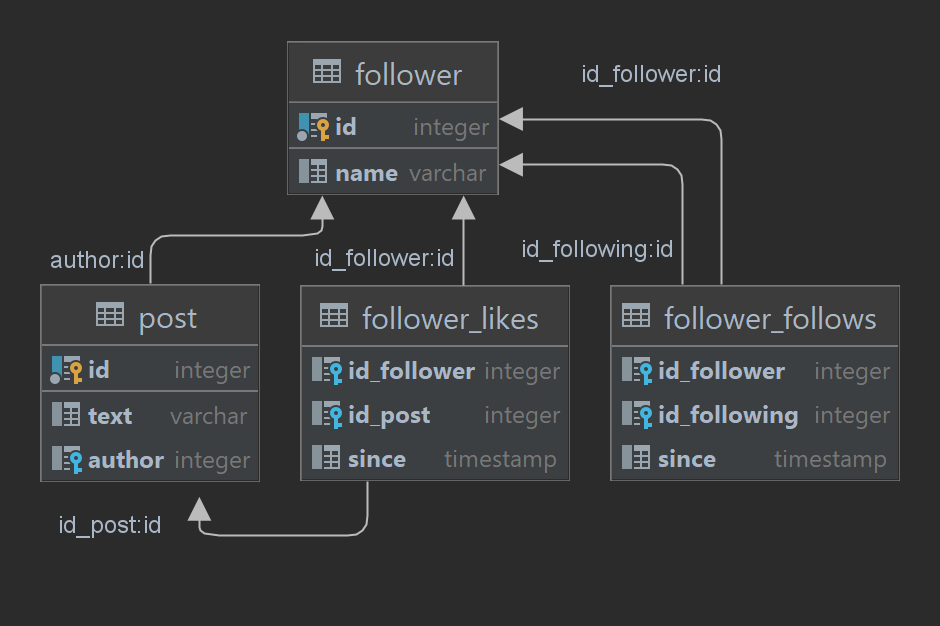
\includegraphics[width=0.7\textwidth]{content/relational-dbms-social-network.png}
    \caption{Relational database for social network}
\end{figure}

As we can see, we need four tables and five foreign keys to describe all relations between two identified entities.
This design can lead to costly joins to answer requests resulting from relationships between entities. For example, we could ask who follows followers who liked someone's post. The query for this example could then look like this:

\begin{listing}[H]
    \begin{minted}
 [
 frame=lines,
 framesep=2mm,
 baselinestretch=1.2,
 bgcolor=LightGray,
 linenos,
 breaklines
 ] {sql}
SELECT followers_of_followers_data.*
FROM post
JOIN follower_likes fl ON post.id = fl.id_post
JOIN follower followers_liked ON fl.id_follower = followers_liked.id
JOIN follower_follows followers_of_followers ON followers_liked.id = followers_of_followers.id_following
JOIN follower followers_of_followers_data ON followers_of_followers.id_follower = followers_of_followers_data.id
WHERE post.id = :post_id
ORDER BY followers_of_followers_data.name;
 \end{minted}
    \caption{SQL query for getting followers of followers who liked a post}
\end{listing}

From the query, we can see that it is barely readable and complex. However, the main problem is performance. The join operations will take more time even for the same request, with more data stored in tables.
Now, we compare the same problem solved using a graph database.

\begin{figure}[H]
    \centering
    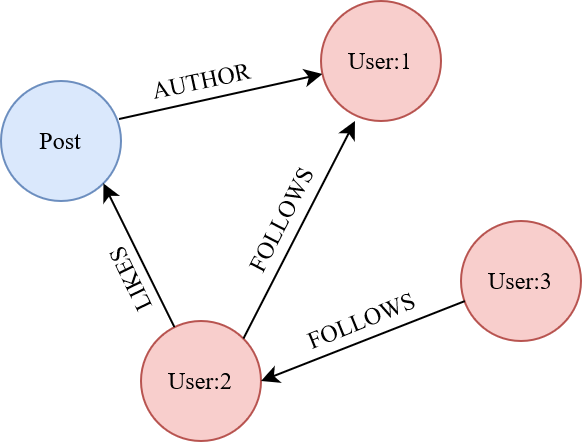
\includegraphics[width=0.8\textwidth]{content/graph_example.png}
    \caption{Graph database for social network}
\end{figure}

As we can see from the picture, each node has one relation or more to other nodes. Furthermore,
the answer to our question from the beginning is already visible if we remind ourselves:
who follows users that liked the post, we can then follow the path in the graph, and as we are going to discover in a moment,
the query to get this information also follows this path.

\begin{listing}[H]
    \begin{minted}
 [
 frame=lines,
 framesep=2mm,
 baselinestretch=1.2,
 bgcolor=LightGray,
 linenos,
 breaklines
 ] {cypher}
 MATCH (:Post {id: {post_id}})-[:LIKES]->(:User)-[:FOLLOWS]->(followers:User) RETURN (followers);
 \end{minted}
    \caption{Cypher query for getting followers of followers who liked a post}
\end{listing}

As promised, the query should not be hard to understand. It is just a quick example of how powerful graph databases can be.

This example was inspired by a blog post from Graham Cox, Introduction to Graph Databases. \cite{cox_introduction_2017}

\section {Native vs. Non-native graph databases}

When dealing with graph databases, we have to look at two main DBMS features: storage and processing.

Storage is how graphs are stored in memory. If the storage is optimized for graphs, like having related nodes close together, we talk about native graph storage when implementation uses other NoSQL storage. Then they are called non-native graph storage.

The second feature mentioned was processing, which refers to how graph databases process database operations. What is meant by that is how the database treats queries and how it handles storage. Native databases use Index-free adjacency for processing.
\cite{chao_graph_2018}

\textbf{Index-free adjacency}: "Native graphs take data that is logically connected via arcs or relationships and hard-wire the physical RAM addresses of these items into the node."
\cite{mccreary_neighborhood_2021} With this in mind, we can now see why graph databases are faster than other types of DBMS.
In traditional RDBMS, looking up a row in another table means that we have to pull an index table representing this relation and then find a path to row in said table.
This behavior leads to another problem in RDBMS because the database uses many indexes to keep data connected, which negatively impacts insert operations.

One more thing we should go through is how the graph database handles writes. Connected data requires strict data integrity.
Graph databases have to create or update nodes themselves and relationships; otherwise, this could result in a corrupted graph, which is almost impossible to fix.
The solution to this problem is to write fully \acrshort{acid}-compliant transactions, ensuring that the database will not become corrupted.
\cite{chao_graph_2018}

\section{Neo4j}

Neo4j is a graph database management system. It is developed by Neo4j, Inc., with its origin in Sweden. \cite{noauthor_company_nodate}
Neo4j is a native graph database, and it is also \acrshort{acid}-compliant. Given these properties, Neo4 uses its custom query language tailored explicitly for querying over graphs,
and its name is Cypher. \cite{noauthor_neo4j_nodate-2}

\section{Cypher}

\textit{Cypher} is a query language created by Neo4j initially for their graph database. Nowadays, it is possible to use Cypher on other graph databases, using "openCypher." \cite{noauthor_resources_nodate}

Its philosophy is to be easily read and understood by developers, database professionals, and business stakeholders.
Its ease of use derives from the fact that it is in accord with how we intuitively describe graphs using diagrams. \cite{robinson_graph_2015}

\subsection{Nodes}

To depict nodes in Cypher, we surround the node with parentheses, e.g., \texttt{(node)}. Parentheses were chosen because they look like circles,
a standard visual representation of nodes in the graph. \cite{noauthor_getting_nodate}

If we need to refer to the node, we can give it a variable like \texttt{(u)} for a user or \texttt{(p)} for a post.
In real-world queries, full names of variables should be used to understand the query better.

With variables, we mentioned the possibility to give a variable name to the nodes, but how can we distinguish two nodes from one to the other.
We can do this by assigning labels to each node. Labels are like tags, which specify certain entities in the graph. If we look back to our example of users and posts,
we can already identify the two labels we would use: \texttt{(p:Post)} and \texttt{(u:User)}.

Specifying labels also has another benefit. When not using labels in a query, the database has to look for all nodes, which can negatively impact the performance of the query.
\cite{noauthor_getting_nodate}

\subsection{Relationship representation}

Relationships between nodes are there to utilize the power of graph databases. They are represented in Cypher using an arrow \texttt{-->}
or \texttt{<--} between two nodes. Additional information, such as by which relationship type are two nodes connected and any properties of the relationship, can be placed in square brackets inside the arrow \texttt{((p:Post)-[:AUTHOR]->(u:User))}. \cite{noauthor_getting_nodate}

The direction of the relationship must be present only while creating the said relationship.
During the traversal of the graph, it is possible to omit the direction by using two dashes (like so: \texttt{--}).
This syntax can make queries more flexible and not force users to know in which directions are relationships stored in the database.

Like with nodes, variables can be used to refer to relationships. If we do not need to reference the relationship later,
we can leave any specification and use an anonymous relationship using two dashes.

\subsection{Nodes and relationship properties}

One thing that was not mentioned yet regarding nodes and relationships is properties. Each node and even each relationship can have one or more properties assigned to them.

Properties are name-value pairs providing additional detail. To represent them in the query, we place them in curly brackets. \cite{noauthor_getting_nodate}
Below is two examples of this usage, one for node and the other for relationship.

\begin{itemize}
    \item {Node property: \texttt{(u:User {nickname: 'mr. Incognito'})}}
    \item {Relationship property: \texttt{-[rel:AUTHOR {posted: 2022-02-05T12:12:20Z}]}}
\end{itemize}

\subsection{Querying with Cypher}

Cypher has few words reserved for specific actions called keywords like most other programming languages. \cite{noauthor_querying_nodate}
First, look at the two most common keywords:
\begin{itemize}
    \item {\texttt{MATCH}: This keyword is what searches for an existing node, relationship, label, property, or pattern in the database. \texttt{MATCH} does work similarly to the \texttt{SELECT} in \acrshort{sql}.}
    \item {\texttt{RETURN}: The \texttt{RETURN} keyword defines what values or results we want to retrieve from the database.
          It is used mainly in search queries as it is not required to be used during write procedures.
          \texttt{RETURN} does utilize the node and relationship variables. If we want to return any results from defined \texttt{MATCH},
          we must specify which nodes, relationships, properties, or patterns we want to return.}
\end{itemize}

\subsection{Create, update, and delete operations}

Besides queries, a proper database system must have methods to create, update or delete data.

The function \texttt{CREATE} is used to insert new data into a graph using Cypher language.
Using \texttt{CREATE}, we can create nodes, relationships, and also patterns. Below are some examples of how \texttt{CREATE} is used and the result. \cite{noauthor_updating_nodate}

\begin{listing}[H]
    \begin{minted}
 [
 frame=lines,
 framesep=2mm,
 baselinestretch=1.2,
 bgcolor=LightGray,
 linenos,
 breaklines
 ] {cypher}
 CREATE (u:User {nickname: "mr. Incognito"})
 RETURN u
 \end{minted}
    \caption{Create a new user with nickname}
\end{listing}

As we can see from examples, we can use the \texttt{RETURN} clause, but it is unnecessary in most cases.

In the following example, we will see \texttt{MATCH} being used before creating a relationship between two nodes.
If we used \texttt{CREATE} right away, we would introduce duplicities of both nodes.

\begin{listing}[H]
    \begin{minted}
 [
 frame=lines,
 framesep=2mm,
 baselinestretch=1.2,
 bgcolor=LightGray,
 linenos,
 breaklines
 ] {cypher}
 MATCH (u:User {nickname: "mr. Incognito"})
 MATCH (p:Post {title: "Hello, world!"})
 CREATE (u)<-[:AUTHOR]-(p)
 \end{minted}
    \caption{Create a new relationship between two nodes}
\end{listing}

There is another way to create this relationship, and we will look at it later in this chapter.

To update data in the database, Cypher uses a \texttt{SET} keyword, which can create or update node or relationship properties.

If we want to delete a node or relationship, we use the \texttt{DELETE} keyword in Cypher language.
This is similar to how \acrshort{sql} \texttt{DELETE} works, but with one exception. If a node is in a relationship
with another node, we cannot delete it because it would create an inconsistent graph, with a potential relationship pointing to nothing. \cite{noauthor_updating_nodate}

We could run two queries to delete the relationship and delete the node itself, but there is a more straightforward solution.
We can use \texttt{DETACH DELETE}, which does detach all relationships from the node before deleting it.

\section{\acrshort{orm}}
\acrshort{orm} stands for an object-relational mapper, which is based on the concept of object-relational mapping.
Object-relational mapping is the idea of writing queries using the object-oriented paradigm.
There are some limitations of what \acrshort{orm} can accomplish. Developers should always consider these limits before using an \acrshort{orm} framework. \cite{mario_hoyos_what_2018}

\noindent Pros:
\begin{itemize}
    \item There is no need to use a second language during software development, \acrshort{sql} is a powerful language, but most developers do not use it too often.
    \item \acrshort{orm} abstracts away from the database system.
    \item It can lead to better performance than writing queries by ourselves.
\end{itemize}
Cons:
\begin{itemize}
    \item If a developer is an \acrshort{sql} power user, he can write queries that will perform better.
    \item Developers have to learn how to use \acrshort{orm} properly.
    \item Developers still need to know how does \acrshort{orm} works under the hood.
\end{itemize}

Using the term \acrshort{orm} with relation to graph databases is not correct. The proper term would be \acrshort{ogm} (object-graph mapper),
but there are a few reasons why we are using \acrshort{orm} instead of \acrshort{ogm} in the name of this thesis. However, please make no mistake,
when discussing \acrshort{orm} involving graph databases, it is, in fact, \acrshort{ogm}.
The main reason is simple: \acrshort{orm} has been around for more than a decade, and developers are familiar with the concept and its challenges.

\section{Conclusion}

In this chapter, we introduced graph databases compared to relational databases. We compared the queries of both types of databases and their differences.
We also studied the differences between native and non-native databases.

The rest of this chapter was focused on Neo4j and Cypher language, where we introduced the basics of this language, like how are relationships and nodes defined,
and base keywords used in Cypher.

In the end, we also adequately introduced the concept of \acrshort{orm} and its relation to \acrshort{ogm}.
